\documentclass{article}
\setcounter{secnumdepth}{4}
\setcounter{tocdepth}{4}

\usepackage{polski}
\usepackage[hidelinks]{hyperref}
\usepackage{caption}
\usepackage{graphicx}
\usepackage{float}

\newcommand{\insertcompanyname}{\textit{ERP System}}
\title{Opis firmy \insertcompanyname}
\author{
    Daniel Staśczak 126816 daniel.stasczak@student.put.poznan.pl
    \\
    Jakub Wiśniewski 126824 jakub.t.wisniewski@student.put.poznan.pl
}
\date{\today}

\begin{document}
    \maketitle

    \newpage
    \tableofcontents
    \listoffigures
    \listoftables

    \newpage
    \section{Charakterystyka ogólna}
        Firma \insertcompanyname, istniejąca od roku 2016, zajmuje się rozwojem i utrzymaniem autorskiego, zintegrowanego systemu informatycznego klasy ERP.

        Użytkownikom oferowane jest pełne wsparcie techniczne, zarówno w kwestii wdrożenia systemu, zapewnienia podstawowych szkoleń, regularnych aktualizacji, jak i obsługi zgłoszeń błędów.

        Przedsiębiorstwo oferuje swoje usługi dla klientów w całej Polsce.

    \newpage
    \section{Struktura organizacyjna}
        Na obecną chwilę, firma składa się sumarycznie z 58 pracowników, podzielonych na niżej wymienione działy:
        \begin{enumerate}
            \item Zarząd (3 osoby) --- odpowiedzialny za strategię rozwoju oraz nadzór całej firmy. Złożony z: prezesa, wiceprezesa oraz dyrektora generalnego firmy.
            \item IT (34 osoby) --- składające się z programistów, devopsów, testerów oraz administratorów; odpowiedzialny za rozwój i utrzymanie systemu pod kątem programistycznym, podzielony na podzespoły realizujące:
            \begin{enumerate}
                \item implementację nowej funkcjonalności głównego systemu, a także wykrywanie i naprawę istniejących błędów (20 osób),
                \item rozbudowę narzędzi wspomagających wsparcie techniczne zapewniane klientom (5 osób),
                \item rozbudowę narzędzi wspomagających działanie samej firmy (3 osób),
                \item rozwój i utrzymanie stron internetowych firmy (3 osób),
                \item lokalną administrację (2 osoby), pracującą w pełnoetatowym systemie dziennym.
            \end{enumerate}
            Nad całym działem czuwa kierownik IT (1 osoba), który pośredniczy w kontakcie z zarządem, odpowiada za przydział zadań i końcową jakość ich realizacji.
            \item Graficy (4 osoby) --- odpowiedzialni za tworzenie ogólnopojętej oprawy graficznej.
            \item Obsługa klienta (5 osób) --- dział odpowiedzialny za bezpośredni kontakt z klientami w kwestii wsparcia pod kątem biznesowym.
            \item Pomoc techniczna (5 osób) --- dział odpowiedzialny za bezpośredni kontakt z klientami w kwestii wsparcia pod kątem technicznym, a także za wsparcie techniczne w firmie.
            \item Dział handlowy (5 osób) --- odpowiedzialny za pozyskiwanie nowych klientów: telefonicznie i poprzez zapewnienie odpowiedniego marketingu firmy. Do ich obowiązków należy również utrzymywanie oficjalnego blogu firmy.
            \item Dział księgowy (2 osoby) --- odpowiedzialny za prowadzenie księgowości w firmie, w tym wszelkie czynności związane z wypłacaniem wynagrodzeń dla pracowników.
        \end{enumerate}
        Dodatkowo wynajmowana jest zewnętrzna firma administracyjna, która pełni podstawowe obowiązki administracyjne w systemie 24/7.

    \newpage
    \section{Siedziba firmy}
        Firma składa się z jednej jednostki zlokalizowanej na drugim piętrze w biurowcu na obrzeżach centrum miasta.
        \subsection{Plan budynku}
            Poniżej przedstawiony jest plan budynku, w którym znajduje się siedziba firmy (ograniczony do odpowiedniego piętra).
            \begin{figure}[H]
                \centering
                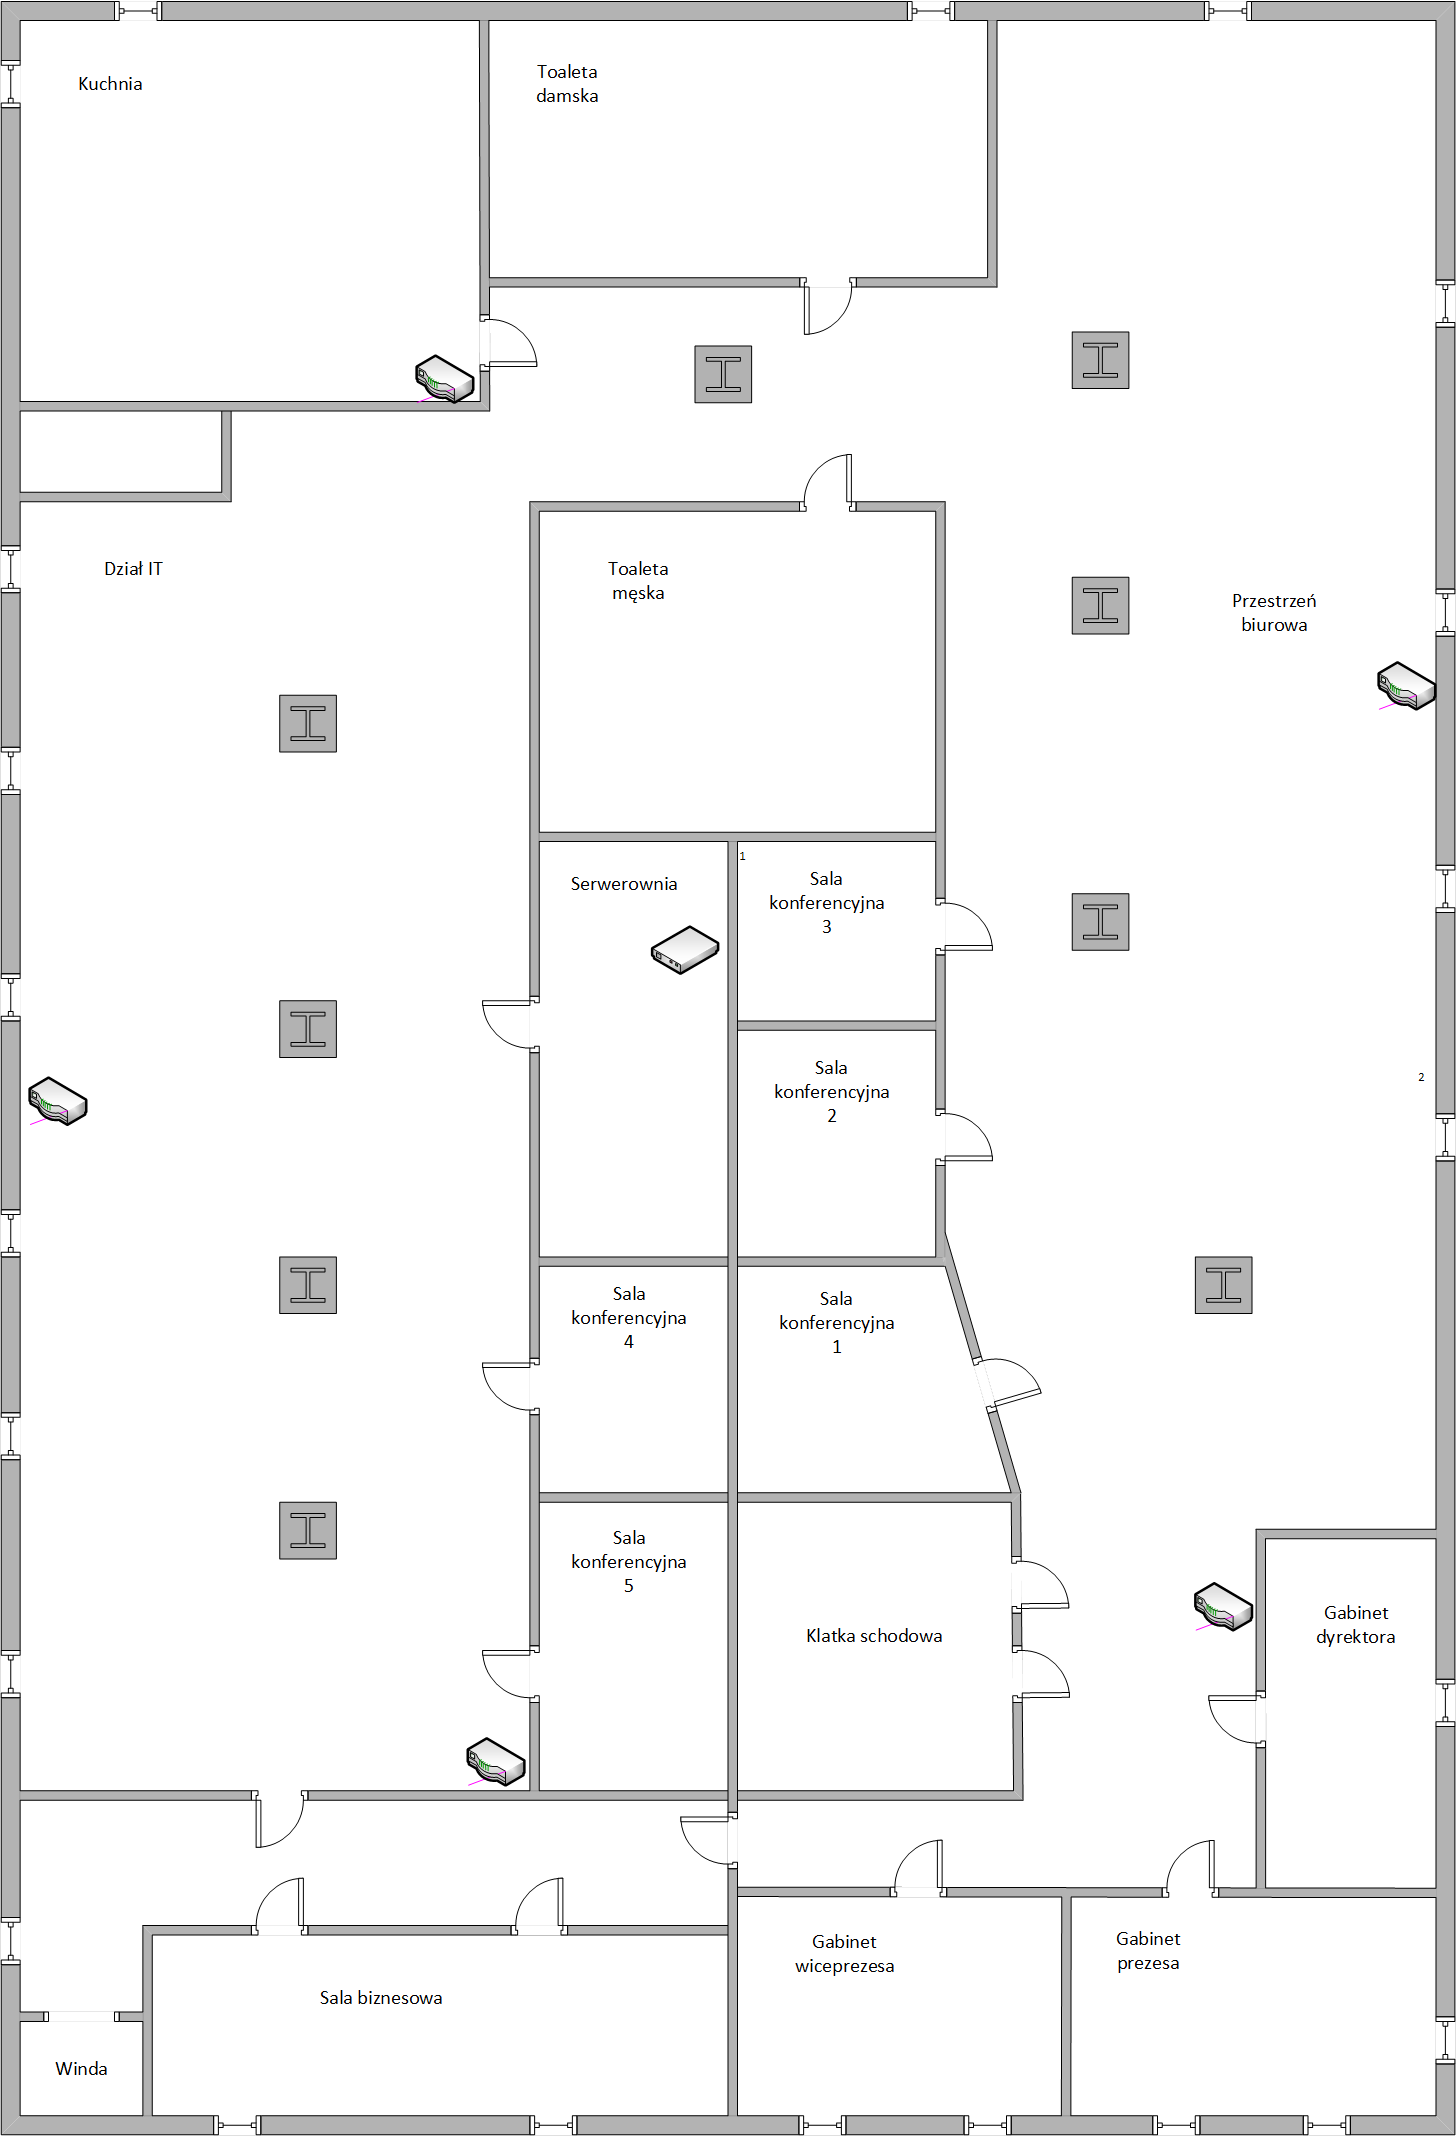
\includegraphics[width=1.0\linewidth]{assets/plan_budynku.png}
                \caption{Plan budynku}
            \end{figure}
        \subsection{Zabezpieczenia lokalu}
            Budynek, w tym sam lokal, monitorowane są systemem kamer oraz chronione przez całodobową ochronę.

            Dostęp do lokalu oraz każdego piętra powyżej i poniżej poziomu 0 (na którym znajduje się portiernia) wymaga karty magnetycznej, przyznawanej w momencie podpisania umowy między firmą a nowym pracownikiem. Karta ta identyfikuje imiennie poszczególnego pracownika oraz zapewnia dostęp jedynie do piętra oraz lokalu, w którym znajduje się firma.

            Domyślnie ów dostęp jest również ograniczony jedynie do dni roboczych, od godziny 6:00 do 20:00, jednakże na specjalny wniosek może on zostać rozszerzony do dodatkowych dni i godzin. Obecnie takim dostępem dysponuje zarząd.

            W wyjątkowych sytuacjach dostępu może również udzielić ochrona.

            Poza tym budynek, w tym sam lokal, wyposażone są w system ochrony przeciwpożarowej w postaci detektorów dymu oraz gaśnicę dostępną na korytarzu każdego piętra.

    \newpage
    \section{Inwentaryzacja zasobów}
        Jako firma zorientowana na usługi z zakresu IT, podstawowym zasobem pracy w biurze jest stanowisko komputerowe, dostępne dla każdego pracownika z osobna: komputery klasy PC lub laptopy.

        Pod względem oprogramowania powszechnym rozwiązaniem jest wykorzystanie rozwiązań firmy Microsoft (system operacyjny, pakiet biurowy), jednakże zarówno architektura głównego systemu informatycznego, jak i narzędzia wykorzystywane przez dział IT, oparte są głównie na darmowych rozwiązaniach Open Source.

        Maszyny serwerowe w większości zlokalizowane są w zewnętrznej firmie, tej samej która odpowiada za zewnętrzne usługi administracyjne --- wyjątkiem jest tu lokalna maszyna, na której pracuje serwer Subversion (repozytorium kodu wszystkich aplikacji rozwijanych przez firmę) oraz FTP (dostępny w miarę potrzeb dla wszystkich pracowników).

        Przez działy obsługi klienta i pomocy technicznej obowiązkowo wykorzystywany jest również system telefonii VoIP.
        \subsection{Sprzęt}
            Na obecną chwilę firma jest w posiadaniu niżej wymienionego sprzętu:
            \begin{table}[H]
                \centering
                \begin{tabular}{ | l | c | }
                    \hline
                    \textbf{Typ} & \textbf{Ilość} \\
                    \hline
                    % 33 IT + 5 OK + 5 PT + + 2 DK + 1 Serwer lokalny
                    Komputer stacjonarny & 46 \\
                    \hline
                    % 3 Zarząd + 1 Kierownik IT + 4 Graficy + 5 DH
                    Laptop klasy biznes & 13 \\
                    \hline
                    % 4 Graficy
                    Tablet graficzny & 4 \\
                    \hline
                    % 5 OK + 5 PT
                    Słuchawki z mikrofonem & 10 \\
                    \hline
                    Router & 1 \\
                    \hline
                    Drukarka sieciowa & 1 \\
                    \hline
                    % Przy założeniu, że będą dwie salki konferencyjne
                    Rzutnik & 7 \\
                    \hline
                    % Na potrzeby backupów
                    Zewnętrzny dysk twardy 1TB & 20 \\
                    \hline
                    % Rzadko używane ze względu na lokalny serwer FTP
                    Pendrive 4GB & 10 \\
                    \hline
                \end{tabular}
                \caption{Wykorzystywany sprzęt}
            \end{table}
        \subsection{Oprogramowanie}
            Na obecną chwilę firma jest w posiadaniu niżej wymienionego \textit{płatnego} oprogramowania:
            \begin{table}[H]
                \centering
                \begin{tabular}{ | l | c | }
                    \hline
                    \textbf{Typ} & \textbf{Ilość} \\
                    \hline
                    % 3 Zarząd + 4 Graficy + 5 OK + 5 PT + 5 DH + + 2 DK + 3 IT + 6 dual boot IT (w tym kierownik)
                    Licencja OEM Windows 10 Enterprise Edition & 33 \\
                    \hline
                    % W zestawie z Windowsem
                    Licencja Microsoft Office 365 & 33 \\
                    \hline
                    Licencja TeamViewer Multi User & 1 \\
                    \hline
                \end{tabular}
                \caption{Wykorzystywane oprogramowanie}
            \end{table}

            Z darmowych rozwiązań wykorzystywane są na miejscu powyższych system operacyjny GNU/Linux (różne dystrybucje) i pakiet biurowy LibreOffice lub OpenOffice.
            Do potrzeb magazynowania i wymiany danych krótkotrwałych wykorzystywany jest lokalny serwer FTP, natomiast jako system ERP stosowany jest autorski system.
        \subsection{Dane}
            System ERP zbudowany jest jako aplikacja webowa, działająca w architekturze klient-serwer.
            Oferowane są dwa warianty:
            \begin{enumerate}
                \item Tańszy, wdrażany całkowicie po stronie klienta, włącznie z bazą danych o dedykowanej strukturze.
                \item Droższy, w którym usługę serwera świadczy firma, włącznie z odpowiedzialnością za całodobowy dostęp do danych, ich bezpieczeństwo oraz regularne kopie zapasowe.
            \end{enumerate}
            W obu wariantach serwer oparty jest o system operacyjny GNU/Linux (dystrybucja CentOS w wersji 5).
            Wykorzystywana baza danych to PostgreSQL w wersji 8.4.

            \subsubsection{Kopie zapasowe}
            Wariant drugi wymaga od firmy magazynowania danych, co wykonywane jest na serwerach zewnętrznych. Cyklicznie co tydzień tworzona jest tam kopia zapasowa bazy danych (jako archiwum typu \texttt{tar.gz}), a co miesiąc najświeższa z nich kopiowana jest dodatkowo na lokalne dyski zewnętrzne (wykorzystywane jest do tego 18 z dostępnych).

            Kopie zapasowe magazynowane na serwerach zewnętrznych są usuwane po trzech miesiącach od daty ich utworzenia, natomiast dane na lokalnych dyskach zewnętrznych nadpisywane są najstarsza przez najnowszą.

            Przestrzeń służąca powyższym współdzielona jest przez dane klientów oraz dane firmy (gdyż dla przypomnienia, firma używa jako systemu ERP aplikacji autorskiej).

            Za lokalne kopie zapasowe odpowiada lokalna administracja.

            Oba z pozostałych dysków zewnętrznych wykorzystywane są do różnych lokalnych potrzeb.

            Dokumenty w formie papierowej magazynowane są w archiwum w biurze. Prowadzona jest polityka tworzenia co najmniej dwóch kopii poszczególnego dokumentu. Nie wszystkie z dokumentów papierowych mają swoje kopie cyfrowe.

            \subsubsection{Lokalna maszyna serwerowa}
            Jak wspomniano we wcześniejszej części rozdziału, lokalnie w firmie znajduje się maszyna serwerowa, na której znajduje się repozytorium kodu Subversion oraz serwer FTP.

            Maszyna zbudowana jest z dwóch dysków twardych po 2TB każdy w układzie RAID 1.

            Za jej utrzymanie odpowiada lokalna administracja.

            \subsubsection{Bezpieczeństwo danych}
            \paragraph{Serwery zewnętrzne}
            Za bezpieczeństwo danych na serwerach zewnętrznych odpowiada zewnętrzna firma administracyjna. Polityka jej działania ogranicza uprawnienia dostępu do minimum: aby otrzymać pełny dostęp administracyjny (za pośrednictwem odpowiedniej konfiguracji komendy \texttt{sudo}) do maszyn serwerowych wymagana jest pisemna zgoda na wzięcie pełnej odpowiedzialności za podejmowane czynności. W przypadku negatywnych skutków takich czynności, zewnętrzna firma administracyjna nie jest upoważniona do ich naprawy.

            Obecnie takim dostępem dysponuje jedynie lokalna administracja oraz, w ograniczonym zakresie (tj. jedynie do wybranych elementów systemu) 3 głównych programistów.

            Oznacza to, że znaczące modyfikacje w systemie, włącznie z procesem wdrożenia nowej wersji rozwijanego systemu na firmowych serwerach zewnętrznych, wymagają działań zewnętrznej firmy administracyjnej lub wyżej wymienionych 5 osób z lokalnego zespołu IT.

            Sam dostęp do w.w. maszyn serwerowych (konto z dostępem realizowanym poprzez protokół SSH, z autoryzacją poprzez hasło) tworzony jest przez zewnętrzną firmę administracyjną na zlecenie upoważnionych osób (zarząd oraz kierownik IT).

            \paragraph{Lokalne elementy systemu}
            Dostęp do innych elementów systemu (lokalna maszyna serwerowa, służbowa poczta e-mail, stacje robocze) realizowany jest przez lokalną administrację.

            Obowiązki te zawierają również odpowiedzialność za generowanie haseł dostępu do tych elementów, które najczęściej składają się z 10 losowych znaków z zakresu znaków alfanumerycznych oraz specjalnych.

            W firmie nie ma jednak określonej żadnej polityki przechowywania haseł: znane są przypadki, gdzie niektórzy pracownicy (głównie spoza działu IT) przechowują je na karteczkach samoprzylepnych przy swoim stanowisku pracy lub zmieniają hasła na prostsze do zapamiętania.

            \paragraph{Dokumenty w formie papierowej}
            Archiwizowane są w szafie zamykanej na klucz.
\end{document}
